%   Il progetto nasce dal template per il frontespizio realizzato da Marco Antonio Corallo, che ringrazio. Seguono alcuni commenti per evidenziare la presenza di alcuni pacchetti che mi sono stati utili per la stesura della tesi. Chiaramente, dipende tutto dal tipo di lavoro che uno vuole eseguire, che determina anche le diverse esigenze. Durante la stesura ho passato molto tempo su siti e forum a cercare di risolvere alcuni probelmi di formattazione, ma in generale Latex è stato piuttosto versatile. 

% Tipo di documento. L'uso di twoside implica che i capitoli inizino sempre con la prima pagina a sinistra, eventualmente lasciando una pagina vuota nel capitolo precedente. Se questa cosa è fastidiosa, è possibile rimuoverlo. 
\documentclass[a4paper, twoside]{article}

% Dimensione dei margini
\usepackage[a4paper,top=2.5cm,bottom=2.5cm,left=2.5cm,right=3cm]{geometry} 
% Dimensione del font
\usepackage[fontsize=12pt]{scrextend}
% Lingua del testo
\usepackage[english,italian]{babel}
% Codifica del testo
\usepackage[utf8]{inputenc} 
% Encoding del testo
\usepackage[T1]{fontenc}
% Permette di generare testo fittizio. Mi è stato utile 
% per capire quale sarebbe stata l'impostazione del 
% testo nella pagina prima che scrivessi un determinato paragrafo
\usepackage{lipsum}
% Per ruotare le immagini
\usepackage{rotating}
% Per modificare l'header delle pagine 
%\usepackage{fancyhdr}
% Librerie matematiche
\usepackage{amssymb}
\usepackage{amsmath}
\usepackage{amsthm}         
\usepackage{float}
% Uso delle immagini
\usepackage{graphicx}
% Uso dei colori
\usepackage[dvipsnames]{xcolor}         
% Uso dei listing per il codice
\usepackage{listings}          
% Per inserire gli hyperlinks tra i vari elementi del testo 
\usepackage{hyperref}
% Diversi tipi di sottolineature
\usepackage[normalem]{ulem}
%per muovere le immagini
\usepackage[export]{adjustbox}
\usepackage{caption}
% \ge= ">="
% \le= "<="
% \cdot= *
\usepackage{subcaption}

%pagine vuote
\usepackage{afterpage}
\newcommand\blankpage{%
    \null
    \thispagestyle{empty}%
    \addtocounter{page}{-1}%
    \newpage}
% Per modificare l'header delle pagine 
\usepackage{fancyhdr}

% -----------------------------------------------------------------


% Modifica lo stile dell'header
\pagestyle{fancy}
\fancyhf{}
\lhead{}
\rhead{}
\rfoot{\thepage}
\fancyfoot[r]{\thepage}
\renewcommand{\headrulewidth}{0pt}
\setlength{\headheight}{14.5pt}

% Rimuove il numero di pagina all'inizio dei capitoli
\fancypagestyle{plain}{
  \fancyfoot{}
  \fancyhead{}
  \renewcommand{\headrulewidth}{0pt}
}

% Forza l'indentazione anche per il primo paragrafo dopo una sezione
\usepackage{indentfirst}

% Definisce l'ampiezza del rientro orizzontale (modificare il valore secondo necessità)
\setlength{\parindent}{1.25cm}

% Definisce la spaziatura verticale tra i paragrafi (modificare il valore secondo necessità)
\setlength{\parskip}{0.5em}

% Stile del codice
\lstdefinestyle{codeStyle}{
    % Colore dei commenti
    commentstyle=\color{teal},
    % Colore delle keyword
    keywordstyle=\color{Magenta},
    % Stile dei numeri di riga
    numberstyle=\tiny\color{gray},
    % Colore delle stringhe
    stringstyle=\color{violet},
    % Dimensione e stile del testo
    basicstyle=\ttfamily\footnotesize,
    % newline solo ai whitespaces
    breakatwhitespace=false,     
    % newline si/no
    breaklines=true,                 
    % Posizione della caption, top/bottom 
    captionpos=b,                    
    % Mantiene gli spazi nel codice, utile per l'indentazione
    keepspaces=true,                 
    % Dove visualizzare i numeri di linea
    numbers=left,                    
    % Distanza tra i numeri di linea
    numbersep=5pt,                  
    % Mostra gli spazi bianchi o meno
    showspaces=false,                
    % Mostra gli spazi bianchi nelle stringhe
    showstringspaces=false,
    % Mostra i tab
    showtabs=false,
    % Dimensione dei tab
    tabsize=2
} \lstset{style=codeStyle}

% Stile di codice per dimensioni maggiori, in cui ho avuto bisogno di un testo più picolo (ad esempio se si vuole inserire del codice che ha linee molto lunghe). Per usare questo stile piuttosto che il precedente, usare 

% \lstset{style=longBlock}
%  % inserire il codice...
% \lstset{style=codeStyle}

% Il secondo comando consente di tornare allo stile precedente 
\lstdefinestyle{longBlock}{
    commentstyle=\color{teal},
    keywordstyle=\color{Magenta},
    numberstyle=\tiny\color{gray},
    stringstyle=\color{violet},
    basicstyle=\ttfamily\scriptsize,
    breakatwhitespace=false,         
    breaklines=true,                 
    captionpos=b,                    
    keepspaces=true,                 
    numbers=left,                    
    numbersep=5pt,                  
    showspaces=false,                
    showstringspaces=false,
    showtabs=false,                  
    tabsize=2
} \lstset{style=codeStyle}

% Togliendo il commento al comando che segue, si inseriscono nella bibliografia anche le fonti presenti in Bibliography.bib ma non citati direttamente con il comando \cite
% \nocite{*}

% Margini prima e dopo blocchi di codice, per avere più distanza
\lstset{aboveskip=20pt,belowskip=20pt}

% Modifica dello stile dei riferimenti, con il testo in cyano
\hypersetup{
    colorlinks=true,
    linkcolor=black,
    filecolor=black,      
    urlcolor=black,
    pdftitle={Overleaf Example},
    pdfpagemode=FullScreen,
    citecolor=black,
    }


% Aggiunti definizioni, teoremi, linea e listing
\newtheorem{definition}{Definizione}[section]
\newtheorem{theorem}{Teorema}[section]
\providecommand*\definitionautorefname{Definizione}
\providecommand*\theoremautorefname{Teorema}
\providecommand*{\listingautorefname}{Listing}
\providecommand*\lstnumberautorefname{Linea}

\raggedbottom

%\newcommand{\cgs}[1]{{\textcolor{brown}[\textcolor{red}{\bf{GS: }}{ \textcolor{brown}{#1]}}}}             
%\newcommand{\cmc}[1]{{\textcolor{blue}[\textcolor{magenta}{\bf{MC: }}{ \textcolor{blue}{#1]}}}}



% -----------------------------------------------------------------
\begin{document}


%\afterpage{\blankpage}
\begin{titlepage}
\begin{figure}[!htb]
    \centering
    
\includegraphics[keepaspectratio=true,scale=0.5]{Images/Frontespizio/Cherubino.jpg}
\end{figure}


\begin{center}
    \LARGE{UNIVERSITÀ DI PISA}
    \vspace{5mm}
    \\ \large{DIPARTIMENTO DI INGEGNERIA INDUSTRIALE}
    \vspace{5mm}
    \\ \LARGE{Laurea Magistrale in Ingegneria Meccanica}
\end{center}

\vspace{15mm}
\begin{center}
        {\bfseries\large\textit{Sviluppo di procedure e sistemi di taratura per \vspace{1.5pt} catene di misura di coppia e forza nel percorso di \vspace{1.5pt} accreditamento UNI EN ISO 17025 di un \vspace{1.5pt} laboratorio prove}}
    
    % Se il titolo è abbastanza corto da stare su una riga, si può usare
    
    % {\LARGE{\bf Un fantastico titolo per la mia tesi!}}
\end{center}
\vspace{30mm}

\begin{minipage}[t]{0.4\textwidth}
	{\large{Relatori:}{\normalsize\vspace{3mm}
	\bf\\ \large{ Prof.   Ciro Santus\\ Ing.    Matteo Nuti} \normalsize\vspace{3mm}}}
\end{minipage}
\hfill
\begin{minipage}[t]{0.4\textwidth}\raggedleft
	{\large{Candidato:}{\normalsize\vspace{3mm} \bf\\ \large{Filippo Magretti}}}
\end{minipage}

\vspace{30mm}
\hrulefill
\\\centering{\large{ANNO ACCADEMICO 2025/2026}}

\end{titlepage}

%----------------------------------------------------------------------------------------
\newpage

%Indice
    \tableofcontents
    \thispagestyle{empty}

    \newpage
% Rimuovere se non si vuole la tabella delle figure
    \listoffigures
    \thispagestyle{empty}

%----------------------------------------------------------------------------------------

    \newpage

	\pagenumbering{arabic}
	\setcounter{page}{1}

    \setcounter{section}{-1}
%----------------------------------------------------------------------------------------
    \blankpage
    \newpage


\section{Introduzione}



\subsection{Contesto di riferimento e obiettivi del tirocinio}



\subsection{I sistemi di prova per trasmissioni meccaniche e il ruolo della metrologia}


%----------------------------------------------------------------------------------------
    \newpage

\section{CAPITOLO 1 - RIFERIMENTI NORMATIVI E METROLOGICI}



\subsection{La metrologia nei laboratori di prova}
La metrologia è la disciplina che riguarda tutti gli aspetti inerenti la misurazione delle grandezze fisiche. 
In particolare, la metrologia tecnico-scientifica ha il compito di rendere disponibili metodologie, unità di misura in modo da garantire l'affidabilità dei processi di misurazione.\par

Con lo scopo di fare chiarezza sui concetti di base, è importante introdurre alcuni termini fondamentali che saranno utilizzati nel corso del lavoro, spesso i quali vengono usati in modo improprio o confusi tra loro.
Innanzitutto è importante chiarire il significato di \textbf{misurazione} e di \textbf{misura}.\\
La \textbf{misurazione} è il processo mediante il quale si ottiene la misura di una grandezza fisica tramite l'utilizzo di opportuni strumenti.\\
La \textbf{misura} è invece il risultato di una misurazione, costituita da: un \textbf{numero}, da una \textbf{incertezza} e da una \textbf{unità di misura}.\par

Fondamentali sono i concetti di \textbf{riproducibilità}, \textbf{ripetibilità} e \textbf{riferibilità}, che costituiscono la qualità di una misurazione all'interno della norma ISO 9001, relativa appunto ai sistemi di gestione per la qualità.\\
Con \textbf{riproducibilità} si intende la possibilità di che persone diverse possano ottenere la stessa misura della stessa grandezza, con risultati confrontabili tra loro.\\
Con \textbf{ripetibilità} si intende la possibilità di ottenere la stessa misura da più misurazioni effettuate dal singolo operatore in tempi differenti ma nelle stesse condizioni.\\
Con \textbf{riferibilità} si intende la possibilità di confrontare il risultato di una misurazione con quello che si ottiene da appropriati campioni di riferimento.\par 

Per quanto riguarda la definizione di \textbf{errore} è importante sottolineare che non esiste una definizione univoca, ma in generale si può definire come la differenza tra il valore misurato e il valore "vero" della grandezza. Si possono comunque distinguere due principali tipi di errore: quello \textbf{casuale} e quello \textbf{sistematico}.\\
Con \textbf{errori casuali} si intendono errori che, per loro natura, al ripetersi delle misurazioni affliggono i valori di misura facendoli oscillare attorno ad un valore pressoché costante (errore di parallasse, o fluttuazioni della stessa grandezza misurata in seguito a variazioni ambientali quali la temperatura ad esempio).\\
Con \textbf{errori sistematici} si intendono invece gli errori di difficile individuazione in quanto si manifestano sempre nello stesso modo, tipicamente provocati dalla strumentazione stessa. \par

Anche i termini di \textbf{precisione} e \textbf{accuratezza} sono spesso confusi tra loro.\\
Con \textbf{precisione} si indica la dispersione dei dati ottenuti dalle misurazioni rispetto al valore "vero" della grandezza misurata, tipicamente espressa tramite  lo \textbf{scarto tipo} detta anche \textbf{deviazione standard sperimentale}, oppure come sinonimo di \textbf{errore relativo}. A questo poi si lega il termine di \textbf{classe di precisione} di uno strumento di misura, ripreso in seguito nel testo.\\
Con \textbf{accuratezza} indica invece la vicinanza tra il valore misurato e il valore "vero" della grandezza misurata.\\
Per rendere più chiara questa distinzione, si può pensare di attribuire queste due definizioni in tutte e quattro le possibili combinazioni per una misura:

\begin{itemize}
    \item precisa e accurata: i valori misurati sono vicini al valore medio e vicini al valore "vero";
    \item precisa ma non accurata: i valori misurati sono vicini al valore medio ma lontani al valore "vero";
    \item non precisa ma accurata: i valori misurati sono lontani al valore medio ma vicini al valore "vero";
    \item non precisa e non accurata: i valori misurati sono lontani sia al valore medio che al valore "vero";
\end{itemize}

\begin{figure}[H]
    \centering
    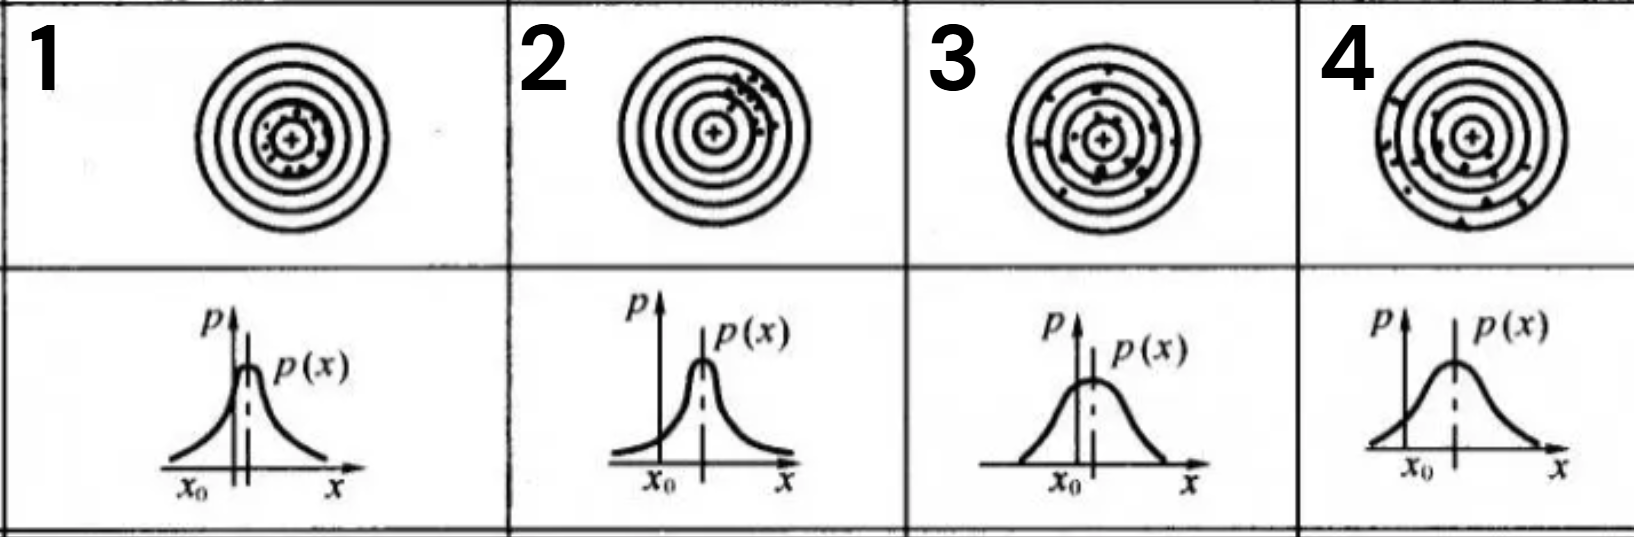
\includegraphics[keepaspectratio=true,scale=0.5]{Images/Capitolo_1/precisione_accuratezza.png}
    \caption{Precisione e accuratezza},
    \label{fig:precisione_accuratezza}
\end{figure}

\par
La questione a questo punto è la seguente: come si può fare una stima dell'errore se non è noto il valore "vero" della grandezza misurata? Qui entra in gioco il concetto di \textbf{incertezza} di una misura, che rappresenta "il risultato della stima che determina l'ampiezza del campo entro il quale il valore vero di un misurando deve trovarsi, generalmente con una data probalità" (come definito nella norma UNI CEI EN ISO 10012 ediz.1993).\\
Il valore "vero" diventa quindi un valore ricavabile in termini statistici dal quale, solo successivamente, è possibile ricavare gli errori, e non un valore di partenza a cui poter fare riferimento sin da subito. Con \textbf{incertezza} si esprime quindi l'intervallo all'interno del quale si trova il valore "vero" con una probabilità elevata.\par

Ora risulta più comprensibile il modo con cui poter scrivere una misura, che come detto è costituita da un numero, da un'incertezza e da un'unità di misura:

\begin{equation}
    \text{Misura} = M_{\text{Valore medio}} \pm U_{\text{Incertezza}} [\text{Unità di misura}]
\end{equation}
dove il valore medio $M$ rappresenta la stima del valore "vero" del misurando e l'incertezza $U$ rappresenta la stima dell'errore tale per cui il valore "vero" ricada all'interno dell'intervallo $[M-U ; M+U]$ con una data probabilità. \par

Per quanto concerne questo elaborato, è importante sottolineare che l'obiettivo principale è quello di sviluppare procedure e sistemi di taratura per \textbf{catene di misura} di coppia e forza, con l'intento di accreditare un laboratorio prove secondo la normativa UNI EN ISO 17025.\\
Rimane solo da definire in modo chiaro cosa si intenda con \textbf{catena di misura}. La catena di misura (o catena metrologica, o catena di riferibilità) è l'insieme di tutti gli elementi che partecipano al processo di misurazione, a partire dallo strumento da tarare fino a un campione di riferimento, chiamato anche \textbf{campione primario}, il quale rappresenta l'unità di misura di riferimento del Sistema Internazionale (SI). In questo modo si costituisce una riferibilità diretta tra lo strumento da tarare e il campione in questione.  


\subsection{1.2	La normativa UNI EN ISO 17025}

Affinché un laboratorio di taratura possa essere accreditato da parte della SINAL (Sistema Nazionale di Accreditamento dei Laboratori), cioè che riceva un riconoscimento da parte di un ente terzo che attesti la competenza tecnica del laboratorio stesso, è necessario che il laboratorio soddisfi i requisiti stabiliti dalla norma UNI EN ISO 17025, che fanno riferimento sia alla capacità operativa che a quella organizzativa del laboratorio.\par

Nel capitolo 4 della norma sono contenuti i requisiti generali di carattere organizzativo e gestionale:

\begin{itemize}
    \item 4.1    Organizzazione
    \item 4.2    Sistema qualità
    \item 4.3    Controllo della documentazione
    \item 4.4    Riesame delle richieste, delle offerte e dei contratti
    \item 4.5    Subappalto delle prove e delle tarature
    \item 4.6    Approvvigionamento di servizi e di forniture
    \item 4.7    Servizi al cliente
    \item 4.8    Reclami
    \item 4.9    Controllo delle attività di prova e/o taratura non conformi
    \item 4.10   Azioni correttive
    \item 4.11   Azioni preventive
    \item 4.12   Controllo delle registrazioni
    \item 4.13   Verifiche ispettive interne
    \item 4.14   Riesami da parte della direzione
\end{itemize}

\noindent
Queste voci non riguardano gli aspetti tecnici, ma concorrono alla qualità e gestione della documentazione, importanti anche dal punto di vista del rapporto tra clienti e fornitori.\par

Nel capitolo 5 della norma sono presi in considerazione invece gli aspetti tecnici, rilevanti per quanto concerne l'affidabilità dei risultati prodotti dal laboratorio, ed è così suddiviso:

\begin{itemize}
    \item 5.1    Generalità
    \item 5.2    Personale
    \item 5.3    Luogo di lavoro e condizioni ambientali
    \item 5.4    Metodi di prova e di taratura e validazione dei metodi
    \item 5.5    Apparecchiature
    \item 5.6    Riferibilità delle misure
    \item 5.7    Campionamento
    \item 5.8    Manipolazione degli oggetti da provare e tarare
    \item 5.9    Assicurazione della qualità dei risultati di prova e di taratura
    \item 5.10   Rappresentazione dei risultati
\end{itemize}

\noindent
Molta importanza è quindi attribuita alla validazione dei metodi di misurazione/taratura (gestione della strumentazione) e alla rintracciabilità metrologica.\\
Per quanto riguarda il primo aspetto sono prescritte procedure per la programmazione delle tarature e per la determinazione dell'incertezza di misura.\\
Per quanto riguarda invece la rintracciabilità metrologica è importante che le misure ottenute siano riferibili ai campioni di riferimento, che ogni taratura della catena di riferibilità sia eseguita in modo adeguato e che sia documentata con evidenza formale, attraverso certificati SIT (Servizio di taratura in Italia) o equivalenti.\par

L'operazione di taratura deve quindi seguire una di queste due tecniche fondamentali:

\begin{itemize}
    \item taratura con una o più misurazioni di una grandezza di valore noto, chiamata \textbf{campione di riferimento};
    \item taratura effettuata con un altro strumento taratore, chiamato \textbf{strumento campione}.
\end{itemize}

\noindent
Occore inoltre che la grandezza (campione) utilizzata, o lo strumento campione, siano caratterizzati da una incertezza inferiore a quella dello strumento da tarare, in questo modo la grandezza associata al campione (oppure il risultato della misurazione effettuata con lo strumento campione) può essere considerata come un valore "vero" per la taratura dello strumento da tarare. \par

In ogni caso il risultato della taratura deve essere rappresentato dallo scostamento tra quanto rilevato e il valore "vero", scostamento calcolato da una o più misurazioni che costituisce l'incertezza di misura assocciata alla taratura stessa, elemento fondamentale per il processo di verifica dell'operazione.\par


\subsection{1.3	Valutazione dell'incertezza di misura}

La “Guide to the expression of Uncertainty in Measurement” (GUM) fornisce
linee guida universali e adottate a livello europeo per valutare l'incertezza nelle misure.\\
L'incertezza di una misura è un parametro che caratterizza la dispersione dei valori ottenuti, e all'interno di questa guida è previsto considerarla come composta da due componenti che differiscono dal metodo di valutazione: l'incertezza di \textbf{tipo A} e l'incertezza di \textbf{tipo B}.\par

L'incertezza di \textbf{tipo A} viene valutata attraverso una serie di ripetute misurazioni, sulle quali vengono effettuate elaborazioni statistiche. Il procedimento da adottare porta al calcolo dello \textbf{scarto tipo}, e risulta utilizzabile anche in sede di taratura, esprimibile come scostamento tra la media ottenuta da un certo numero di prove e il valore "vero" di riferimento fornito da un campione o da uno strumento campione. I risultati di questo procedimento sono quelli tipicamente ripotati nei certificati di taratura.\par

La procedura per la valutazione dell'incertezza di tipo A prevede di effettuare $N$ misurazioni e di seguire i successivi step:

\begin{itemize}
    \item calcolo della \text{media} come media aritmetica $m$ dei valori misurati
    
    \begin{equation}
    m = \frac{1}{N} \sum_{i=1}^{N} x_i
    \end{equation}

    \item calcolo degli \textbf{scarti} $s_i$ dei valori misurati rispetto alla media
   
    \begin{equation}
    s_i = x_i - m
    \end{equation}

    \item calcolo dello \textbf{scarto tipo} $s$ come stima della deviazione standard sperimentale di una distribuzione ipoteticamente gaussiana
    
    \begin{equation}
    s = \sqrt{\frac{1}{N-1} \sum_{i=1}^{N} s_i^2}
    \end{equation}

\end{itemize}

Occorre considerare nel calcolo della misurazione anche un altro contributo dovuto alla \textbf{incertezza diripetibilità}, classificabile come incertezzadi tipo A, che viene così calcolata:

\begin{itemize}
    \item calcolo della \textbf{media} $m$ calcolata su $N$ misurazioni come media aritmetica dei valori misurati;
    \item calcolo dello \textbf{scarto tipo} $s$ come illustrato in precedenza;
    \item calcolo della \textbf{deviazione standard della media} $s_m$ andando a dividere lo scarto tipo $s$ per la radice quadrata del numero di misurazioni $N$ effettuate
    
    \begin{equation}
    s_m = \frac{s}{\sqrt{N}}
    \end{equation}

\end{itemize}

L'incertezza di \textbf{tipo B} viene valutata invece tramite modalità che non necessitano di misurazioni ripetute, e il suo calcolo parte dalla conoscenza dell'entità massima della variazione casuale \textbf{$a$} di una grandezza, la quale tipicamente è simmetrica rispetto a zero, assumendo quindi valori compresi nell'intervallo $[-a ; a]$. Il valore \textbf{$a$} è ottenuto da report informativi, certificati di taratura, risultati sperimentali, in sostanza da conoscenze a priori del contesto in cui si opera.\\
Stabilito il valore di $a$, in seguito a una ipotesi di distribuzione statistica della grandezza misurata all'interno dell'intervallo $[-a ; a]$, è possibile calcolare l'incertezza di tipo B $u$ nel modo seguente:

\begin{itemize}
    \item nel caso di variabili casuali, si ipotizza una \textbf{distribuzione rettangolare}, la cui deviazione standard è pari a
    
    \begin{equation}
    u = \frac{a}{\sqrt{3}}
    \end{equation}

     Questa ipotesi viene fatta nei casi in cui non si hanno informazioni sufficienti per poter fare ipotesi più specifiche riguardo alla distribuzione della grandezza misurata.
\end{itemize}

Una volta calcolate le due componenti A e B, è possibile calcolare una combinazione di queste due incertezze, calcolando così una incertezza risultante, detta \textbf{incertezza tipo}.\par

Al termine di un processo di misurazione, ottenuti $n$ valori di deviazione standard $u_1, u_2, ..., u_n$ associati a $n$ fonti di incertezza, l'\textbf{incertezza tipo} $u$ è data dalla loro somma quadratica, che si basa sull'ipotesi di indipendenza tra le fonti di incertezza:

\begin{equation}
u = \sqrt{u_1^2 + u_2^2 + ... + u_n^2}
\end{equation}

Successivamente occore determinare l'\textbf{equazione della misura}, che lega la grandezza misurata $Y$ alle grandezze di ingresso $X_1, X_2, ..., X_n$ che influenzano la misura. L'eventuale mancanza di informazioni relativa a tali grandezze di ingresso, alle loro relative misure ed incertezze, e alla relazione stessa che le lega alla gradezza misurata, determinerebbe una ulteriore fonte di incertezza, tipica degli ambienti di sperimentazione scientifica e meno usuale in ambito industriale.\par
Ipotizzando di conoscere l'equazione della misura, è possibile calcolare la \textbf{legge di propagazione dell'incertezza}, che corrisponde alla legge di propagazione degli errori, riportata nell'appendice 1, che consente di calcolare la stima della varianza (ossia il quadrato della deviazione standard) come una combinazione lineare delle varianze associate alle grandezze di ingresso $X_1, X_2, ..., X_n$, ciascuna pesata con il quadrato del coefficiente di sensibilità $c_i$ che rappresenta la derivata parziale della grandezza misurata $Y$ rispetto alla grandezza di ingresso $X_i$.\par
Calcolandone poi la radice quadrata si ottiene l'\textbf{incertezza tipo composta} $u_c$, risultato della propagazione delle varie incertezze.

\begin{itemize}
    \item Approccio GUM
    \item Incertezze di tipo A e di tipo B
    \item Propagazione dell’incertezza
    \item Budget di incertezza
\end{itemize}


%----------------------------------------------------------------------------------------
    \newpage

\section{CAPITOLO 2 - DESCRIZIONE DEI SISTEMI DI PROVA}



\subsection{Banco prova ingranaggi}



\begin{itemize}
    \item Architettura del sistema
    \item Catene di misura della coppia
    \item Torsiometri utilizzati
    \item Sistema di acquisisizione dati
\end{itemize}



\subsection{Macchina per test STBF}



\begin{itemize}
    \item Descrizione dell'attrezzatura di afferraggio
    \item Cella di carico
    \item Ponti estensimetrici
    \item Sistema di acquisisizione dati
\end{itemize}


%----------------------------------------------------------------------------------------
    \newpage

\section{CAPITOLO 3 - SISTEMA DI TARATURA DEI TORSIOMETRI}



\subsection{Analisi delle esigenze metrologiche}



\subsection{Progettaazione del sistema di taratura}



\begin{itemize}
    \item Scelta dei pesi certificati
    \item configurazione Meccanica
    \item braggio di leva e generazione della coppia
\end{itemize}



\subsection{Realizzazione e collaudo}



\subsection{Procedura di taratura}



\subsection{Analisi dei risultati sperimentali}



\begin{itemize}
    \item Linearità
    \item Ripetibiilità
    \item Isteresi   
\end{itemize}
    

%----------------------------------------------------------------------------------------
    \newpage

\section{CAPITOLO 4 - SISTEMA DI VERIFICA DI CELLA DI CARICO E PONTI ESTENSIMETRICI}



\subsection{Analisi della catena di misura della forza}



\subsection{Progettazone del sistema di verifica}



\subsection{Realizzazione e collaudo}



\subsection{Procedura di verifica}



\subsection{Analisi delle prestazioni metrologiche}


%----------------------------------------------------------------------------------------
    \newpage

\section{CAPITOLO 5 - Confronto con requisiti ISO 17025}



\subsection{Adeguatezza metrologica}



\subsection{Margini di miglioramento}


%----------------------------------------------------------------------------------------
    \newpage

\section{CAPITOLO 6 - GESTIONE DELLA STRUMENTAZIONE E PROCESSI DI QUALITÀ}



\subsection{Procedure di gestione della stumentazione}



\subsection{Tracciabilità metrologica}



\subsection{Piano di taratura periodica}



\subsection{Integrazione nel sistema qualità aziendale}


%----------------------------------------------------------------------------------------
    \newpage

\section{CAPITOLO 7 - CONCLUSIONI}
%----------------------------------------------------------------------------------------
    \newpage

\section{APPENDICI}
%----------------------------------------------------------------------------------------



\end{document}
